
\documentclass{beamer}

\usepackage[T1]{fontenc}
\usepackage[utf8]{inputenc}
\usepackage[english]{babel}
\usepackage{lmodern}
% \usepackage{forloop}
\usepackage{multicol}
\usepackage{animate}
\usepackage{default}
\usepackage{listing}

\usepackage[list=true]{subcaption}
\captionsetup{compatibility=false}
\usepackage{etex}


\usepackage{tikz}
% \usepackage{polyglossia}
% \usepackage{listings}
% \usepackage{ulem}
% \usepackage{multicol}

% \setbeamertemplate{navigation symbols}{}
% \setbeamertemplate{sidebar right}{}
% \setbeamertemplate{footline}{\hfill\insertframenumber{} | \inserttotalframenumber}


% \newcommand{\myline}{\par
%     \kern0.5pt
%     \hrule height 0.8pt
%     \kern0.5pt
% }

\usecolortheme{cormorant}
\useoutertheme{infolines}



\title[Présentation]{H4ck 1n TN}
\subtitle{Présentation du club}
\author[H4ck1nTN]{
	Gabrielle TOULET MORLANNE (Secrétaire)
\and \\
Benoît TALLANDIER (Trésorier)
\and \\
Olivier DAUTRICOURT (Président)
}

\institute[HiT]{Ceten -- TELECOM Nancy}
\date{\today}
\logo{
\includegraphics[width=1.3cm]{logo.png}}

\begin{document}


\begin{frame}
\titlepage
\end{frame} 


\begin{frame}{Objectifs du club}
	\begin{itemize}
		\item Vous former à la sécurité informatique
		\item Apprendre des choses qu'on ne voit pas forcément à Télécom
		\item Partager ses connaissances
		\item S'amuser :)
	\end{itemize}
	
\end{frame}


\begin{frame}{Ce qu'on y fait}
	\begin{itemize}
		\item Une présentation toutes les 2/3 semaines
		\item Des challenges (CTF)
		\item Des évènements (Confs, Ateliers, CTFs, ...)
		\item Ce que vous voulez 
	\end{itemize}
\end{frame}

\begin{frame}{Informations utiles}
	\begin{itemize}
		\item Site du club: https://hackintn.telecomnancy.net
		\item Github du club: github.com/HackInTN
		\item Canal IRC : \#HackInTN sur @freenode
	\end{itemize}
\end{frame}

\begin{frame} {Le GreHack}
	\begin{itemize}
		\item Quoi : Conférences ethical hacking \& workshops \& CTF 
		\item Quand : Vendredi 18 -> Samedi 19  novembre
		\item Où : Ensimag, Grenoble 
		\item plus d'info sur grehack.fr
	\end{itemize}
\end{frame}

\begin{frame} {Le GreHack}
	\begin{itemize}
		\item Confs de 2015 dispo sur youtube
		\item Tout le monde ne pourra pas venir ! (2-3 places)
		\item A gagner: Des goodies, de l'expèrience , 5 points CIPA
	\end{itemize}
\end{frame}

\begin{frame}{Sites d'apprentissage}
	\begin{itemize}
		\item root-me.org (Site de challenge en tout genre\\
		Cracking, Web, Crypto, Réseau...)
			
		\item overthewire.org (Site de challenges orientés systeme)
		
		\item github.com/ctfs (write-ups des CTF passés)
		
		\item canyouhack.it
	\end{itemize}
\end{frame}

\begin{frame}{Medias/(SEC | IT)}
	\begin{itemize}
		\item Misc (Magazine)
		\item HackerNews
		\item blog.codinghorror.com
	\end{itemize}
\end{frame}

\begin{frame}{Libre/GNU/tux/rainbow}
	\centerline{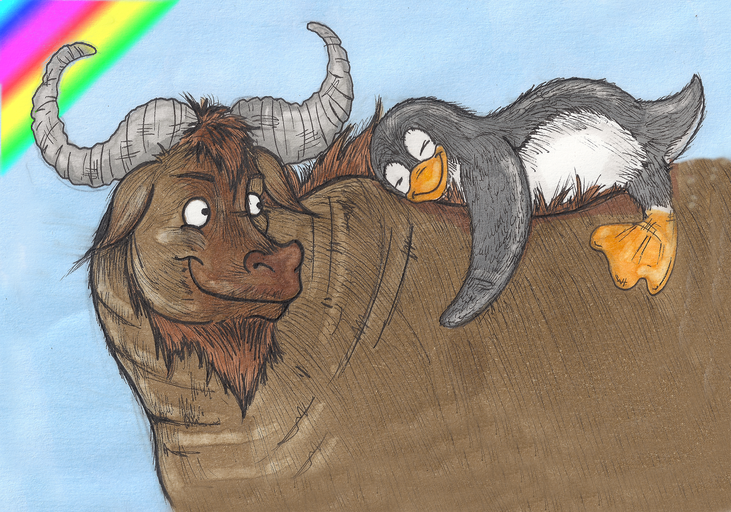
\includegraphics[scale=2.1]{libre2.png}}
\end{frame}

\begin{frame}{Medias/Libre}
	\begin{itemize}
		\item framasoft.org 
		\item standblog.org
		\item laquadrature.net
	\end{itemize}
\end{frame}

\begin{frame}{Libre/GNU/tux/rainbow}
	\centerline{
\includegraphics[scale=0.6]{libre1.png}}
\end{frame}

\begin{frame}{Distributions}
	\begin{itemize}
		\item Kali Linux (Distribution Linux orientée pentesting)
		
		\item Tails (axé sécu/anonymat)
		
		\item Quebes (Basé sur de la virtualisation)
		
		\item Blackbox ...
	\end{itemize}
\end{frame}

\begin{frame}{Quelques outils}
	\begin{itemize}
		\item nmap
		\item wireshark, tcpdump, Dsniff
		\item john
		\item nikto, owasp zap
		\item aircrack-ng (wifite), btscanner/bluesnarfer
		\item Metasploit Framework
		\item SEToolkit
	\end{itemize}
\end{frame}

\begin{frame}{Quelques outils}
	\begin{itemize}
		\item strace, ltrace
		\item gdb, valgrind
		\item radare2, IDA (désassembleur/analyseur de code)
		\item binwalk
	\end{itemize}
\end{frame}


\begin{frame}
	\centerline{
\includegraphics[scale=0.9]{rtfm.png}}
\end{frame}


\begin{frame} 
	\begin{itemize}
		\item Des Questions ?
		\item Write up (challlenge de rentrée) 
	\end{itemize}
\end{frame}


\end{document}
